
% Default to the notebook output style

    


% Inherit from the specified cell style.




    
\documentclass[11pt]{article}

    
    
    \usepackage[T1]{fontenc}
    % Nicer default font (+ math font) than Computer Modern for most use cases
    \usepackage{mathpazo}

    % Basic figure setup, for now with no caption control since it's done
    % automatically by Pandoc (which extracts ![](path) syntax from Markdown).
    \usepackage{graphicx}
    % We will generate all images so they have a width \maxwidth. This means
    % that they will get their normal width if they fit onto the page, but
    % are scaled down if they would overflow the margins.
    \makeatletter
    \def\maxwidth{\ifdim\Gin@nat@width>\linewidth\linewidth
    \else\Gin@nat@width\fi}
    \makeatother
    \let\Oldincludegraphics\includegraphics
    % Set max figure width to be 80% of text width, for now hardcoded.
    \renewcommand{\includegraphics}[1]{\Oldincludegraphics[width=.8\maxwidth]{#1}}
    % Ensure that by default, figures have no caption (until we provide a
    % proper Figure object with a Caption API and a way to capture that
    % in the conversion process - todo).
    \usepackage{caption}
    \DeclareCaptionLabelFormat{nolabel}{}
    \captionsetup{labelformat=nolabel}

    \usepackage{adjustbox} % Used to constrain images to a maximum size 
    \usepackage{xcolor} % Allow colors to be defined
    \usepackage{enumerate} % Needed for markdown enumerations to work
    \usepackage{geometry} % Used to adjust the document margins
    \usepackage{amsmath} % Equations
    \usepackage{amssymb} % Equations
    \usepackage{textcomp} % defines textquotesingle
    % Hack from http://tex.stackexchange.com/a/47451/13684:
    \AtBeginDocument{%
        \def\PYZsq{\textquotesingle}% Upright quotes in Pygmentized code
    }
    \usepackage{upquote} % Upright quotes for verbatim code
    \usepackage{eurosym} % defines \euro
    \usepackage[mathletters]{ucs} % Extended unicode (utf-8) support
    \usepackage[utf8x]{inputenc} % Allow utf-8 characters in the tex document
    \usepackage{fancyvrb} % verbatim replacement that allows latex
    \usepackage{grffile} % extends the file name processing of package graphics 
                         % to support a larger range 
    % The hyperref package gives us a pdf with properly built
    % internal navigation ('pdf bookmarks' for the table of contents,
    % internal cross-reference links, web links for URLs, etc.)
    \usepackage{hyperref}
    \usepackage{longtable} % longtable support required by pandoc >1.10
    \usepackage{booktabs}  % table support for pandoc > 1.12.2
    \usepackage[inline]{enumitem} % IRkernel/repr support (it uses the enumerate* environment)
    \usepackage[normalem]{ulem} % ulem is needed to support strikethroughs (\sout)
                                % normalem makes italics be italics, not underlines
    

    
    
    % Colors for the hyperref package
    \definecolor{urlcolor}{rgb}{0,.145,.698}
    \definecolor{linkcolor}{rgb}{.71,0.21,0.01}
    \definecolor{citecolor}{rgb}{.12,.54,.11}

    % ANSI colors
    \definecolor{ansi-black}{HTML}{3E424D}
    \definecolor{ansi-black-intense}{HTML}{282C36}
    \definecolor{ansi-red}{HTML}{E75C58}
    \definecolor{ansi-red-intense}{HTML}{B22B31}
    \definecolor{ansi-green}{HTML}{00A250}
    \definecolor{ansi-green-intense}{HTML}{007427}
    \definecolor{ansi-yellow}{HTML}{DDB62B}
    \definecolor{ansi-yellow-intense}{HTML}{B27D12}
    \definecolor{ansi-blue}{HTML}{208FFB}
    \definecolor{ansi-blue-intense}{HTML}{0065CA}
    \definecolor{ansi-magenta}{HTML}{D160C4}
    \definecolor{ansi-magenta-intense}{HTML}{A03196}
    \definecolor{ansi-cyan}{HTML}{60C6C8}
    \definecolor{ansi-cyan-intense}{HTML}{258F8F}
    \definecolor{ansi-white}{HTML}{C5C1B4}
    \definecolor{ansi-white-intense}{HTML}{A1A6B2}

    % commands and environments needed by pandoc snippets
    % extracted from the output of `pandoc -s`
    \providecommand{\tightlist}{%
      \setlength{\itemsep}{0pt}\setlength{\parskip}{0pt}}
    \DefineVerbatimEnvironment{Highlighting}{Verbatim}{commandchars=\\\{\}}
    % Add ',fontsize=\small' for more characters per line
    \newenvironment{Shaded}{}{}
    \newcommand{\KeywordTok}[1]{\textcolor[rgb]{0.00,0.44,0.13}{\textbf{{#1}}}}
    \newcommand{\DataTypeTok}[1]{\textcolor[rgb]{0.56,0.13,0.00}{{#1}}}
    \newcommand{\DecValTok}[1]{\textcolor[rgb]{0.25,0.63,0.44}{{#1}}}
    \newcommand{\BaseNTok}[1]{\textcolor[rgb]{0.25,0.63,0.44}{{#1}}}
    \newcommand{\FloatTok}[1]{\textcolor[rgb]{0.25,0.63,0.44}{{#1}}}
    \newcommand{\CharTok}[1]{\textcolor[rgb]{0.25,0.44,0.63}{{#1}}}
    \newcommand{\StringTok}[1]{\textcolor[rgb]{0.25,0.44,0.63}{{#1}}}
    \newcommand{\CommentTok}[1]{\textcolor[rgb]{0.38,0.63,0.69}{\textit{{#1}}}}
    \newcommand{\OtherTok}[1]{\textcolor[rgb]{0.00,0.44,0.13}{{#1}}}
    \newcommand{\AlertTok}[1]{\textcolor[rgb]{1.00,0.00,0.00}{\textbf{{#1}}}}
    \newcommand{\FunctionTok}[1]{\textcolor[rgb]{0.02,0.16,0.49}{{#1}}}
    \newcommand{\RegionMarkerTok}[1]{{#1}}
    \newcommand{\ErrorTok}[1]{\textcolor[rgb]{1.00,0.00,0.00}{\textbf{{#1}}}}
    \newcommand{\NormalTok}[1]{{#1}}
    
    % Additional commands for more recent versions of Pandoc
    \newcommand{\ConstantTok}[1]{\textcolor[rgb]{0.53,0.00,0.00}{{#1}}}
    \newcommand{\SpecialCharTok}[1]{\textcolor[rgb]{0.25,0.44,0.63}{{#1}}}
    \newcommand{\VerbatimStringTok}[1]{\textcolor[rgb]{0.25,0.44,0.63}{{#1}}}
    \newcommand{\SpecialStringTok}[1]{\textcolor[rgb]{0.73,0.40,0.53}{{#1}}}
    \newcommand{\ImportTok}[1]{{#1}}
    \newcommand{\DocumentationTok}[1]{\textcolor[rgb]{0.73,0.13,0.13}{\textit{{#1}}}}
    \newcommand{\AnnotationTok}[1]{\textcolor[rgb]{0.38,0.63,0.69}{\textbf{\textit{{#1}}}}}
    \newcommand{\CommentVarTok}[1]{\textcolor[rgb]{0.38,0.63,0.69}{\textbf{\textit{{#1}}}}}
    \newcommand{\VariableTok}[1]{\textcolor[rgb]{0.10,0.09,0.49}{{#1}}}
    \newcommand{\ControlFlowTok}[1]{\textcolor[rgb]{0.00,0.44,0.13}{\textbf{{#1}}}}
    \newcommand{\OperatorTok}[1]{\textcolor[rgb]{0.40,0.40,0.40}{{#1}}}
    \newcommand{\BuiltInTok}[1]{{#1}}
    \newcommand{\ExtensionTok}[1]{{#1}}
    \newcommand{\PreprocessorTok}[1]{\textcolor[rgb]{0.74,0.48,0.00}{{#1}}}
    \newcommand{\AttributeTok}[1]{\textcolor[rgb]{0.49,0.56,0.16}{{#1}}}
    \newcommand{\InformationTok}[1]{\textcolor[rgb]{0.38,0.63,0.69}{\textbf{\textit{{#1}}}}}
    \newcommand{\WarningTok}[1]{\textcolor[rgb]{0.38,0.63,0.69}{\textbf{\textit{{#1}}}}}
    
    
    % Define a nice break command that doesn't care if a line doesn't already
    % exist.
    \def\br{\hspace*{\fill} \\* }
    % Math Jax compatability definitions
    \def\gt{>}
    \def\lt{<}
    % Document parameters
    \title{Assignment 4}
    
    
    

    % Pygments definitions
    
\makeatletter
\def\PY@reset{\let\PY@it=\relax \let\PY@bf=\relax%
    \let\PY@ul=\relax \let\PY@tc=\relax%
    \let\PY@bc=\relax \let\PY@ff=\relax}
\def\PY@tok#1{\csname PY@tok@#1\endcsname}
\def\PY@toks#1+{\ifx\relax#1\empty\else%
    \PY@tok{#1}\expandafter\PY@toks\fi}
\def\PY@do#1{\PY@bc{\PY@tc{\PY@ul{%
    \PY@it{\PY@bf{\PY@ff{#1}}}}}}}
\def\PY#1#2{\PY@reset\PY@toks#1+\relax+\PY@do{#2}}

\expandafter\def\csname PY@tok@w\endcsname{\def\PY@tc##1{\textcolor[rgb]{0.73,0.73,0.73}{##1}}}
\expandafter\def\csname PY@tok@c\endcsname{\let\PY@it=\textit\def\PY@tc##1{\textcolor[rgb]{0.25,0.50,0.50}{##1}}}
\expandafter\def\csname PY@tok@cp\endcsname{\def\PY@tc##1{\textcolor[rgb]{0.74,0.48,0.00}{##1}}}
\expandafter\def\csname PY@tok@k\endcsname{\let\PY@bf=\textbf\def\PY@tc##1{\textcolor[rgb]{0.00,0.50,0.00}{##1}}}
\expandafter\def\csname PY@tok@kp\endcsname{\def\PY@tc##1{\textcolor[rgb]{0.00,0.50,0.00}{##1}}}
\expandafter\def\csname PY@tok@kt\endcsname{\def\PY@tc##1{\textcolor[rgb]{0.69,0.00,0.25}{##1}}}
\expandafter\def\csname PY@tok@o\endcsname{\def\PY@tc##1{\textcolor[rgb]{0.40,0.40,0.40}{##1}}}
\expandafter\def\csname PY@tok@ow\endcsname{\let\PY@bf=\textbf\def\PY@tc##1{\textcolor[rgb]{0.67,0.13,1.00}{##1}}}
\expandafter\def\csname PY@tok@nb\endcsname{\def\PY@tc##1{\textcolor[rgb]{0.00,0.50,0.00}{##1}}}
\expandafter\def\csname PY@tok@nf\endcsname{\def\PY@tc##1{\textcolor[rgb]{0.00,0.00,1.00}{##1}}}
\expandafter\def\csname PY@tok@nc\endcsname{\let\PY@bf=\textbf\def\PY@tc##1{\textcolor[rgb]{0.00,0.00,1.00}{##1}}}
\expandafter\def\csname PY@tok@nn\endcsname{\let\PY@bf=\textbf\def\PY@tc##1{\textcolor[rgb]{0.00,0.00,1.00}{##1}}}
\expandafter\def\csname PY@tok@ne\endcsname{\let\PY@bf=\textbf\def\PY@tc##1{\textcolor[rgb]{0.82,0.25,0.23}{##1}}}
\expandafter\def\csname PY@tok@nv\endcsname{\def\PY@tc##1{\textcolor[rgb]{0.10,0.09,0.49}{##1}}}
\expandafter\def\csname PY@tok@no\endcsname{\def\PY@tc##1{\textcolor[rgb]{0.53,0.00,0.00}{##1}}}
\expandafter\def\csname PY@tok@nl\endcsname{\def\PY@tc##1{\textcolor[rgb]{0.63,0.63,0.00}{##1}}}
\expandafter\def\csname PY@tok@ni\endcsname{\let\PY@bf=\textbf\def\PY@tc##1{\textcolor[rgb]{0.60,0.60,0.60}{##1}}}
\expandafter\def\csname PY@tok@na\endcsname{\def\PY@tc##1{\textcolor[rgb]{0.49,0.56,0.16}{##1}}}
\expandafter\def\csname PY@tok@nt\endcsname{\let\PY@bf=\textbf\def\PY@tc##1{\textcolor[rgb]{0.00,0.50,0.00}{##1}}}
\expandafter\def\csname PY@tok@nd\endcsname{\def\PY@tc##1{\textcolor[rgb]{0.67,0.13,1.00}{##1}}}
\expandafter\def\csname PY@tok@s\endcsname{\def\PY@tc##1{\textcolor[rgb]{0.73,0.13,0.13}{##1}}}
\expandafter\def\csname PY@tok@sd\endcsname{\let\PY@it=\textit\def\PY@tc##1{\textcolor[rgb]{0.73,0.13,0.13}{##1}}}
\expandafter\def\csname PY@tok@si\endcsname{\let\PY@bf=\textbf\def\PY@tc##1{\textcolor[rgb]{0.73,0.40,0.53}{##1}}}
\expandafter\def\csname PY@tok@se\endcsname{\let\PY@bf=\textbf\def\PY@tc##1{\textcolor[rgb]{0.73,0.40,0.13}{##1}}}
\expandafter\def\csname PY@tok@sr\endcsname{\def\PY@tc##1{\textcolor[rgb]{0.73,0.40,0.53}{##1}}}
\expandafter\def\csname PY@tok@ss\endcsname{\def\PY@tc##1{\textcolor[rgb]{0.10,0.09,0.49}{##1}}}
\expandafter\def\csname PY@tok@sx\endcsname{\def\PY@tc##1{\textcolor[rgb]{0.00,0.50,0.00}{##1}}}
\expandafter\def\csname PY@tok@m\endcsname{\def\PY@tc##1{\textcolor[rgb]{0.40,0.40,0.40}{##1}}}
\expandafter\def\csname PY@tok@gh\endcsname{\let\PY@bf=\textbf\def\PY@tc##1{\textcolor[rgb]{0.00,0.00,0.50}{##1}}}
\expandafter\def\csname PY@tok@gu\endcsname{\let\PY@bf=\textbf\def\PY@tc##1{\textcolor[rgb]{0.50,0.00,0.50}{##1}}}
\expandafter\def\csname PY@tok@gd\endcsname{\def\PY@tc##1{\textcolor[rgb]{0.63,0.00,0.00}{##1}}}
\expandafter\def\csname PY@tok@gi\endcsname{\def\PY@tc##1{\textcolor[rgb]{0.00,0.63,0.00}{##1}}}
\expandafter\def\csname PY@tok@gr\endcsname{\def\PY@tc##1{\textcolor[rgb]{1.00,0.00,0.00}{##1}}}
\expandafter\def\csname PY@tok@ge\endcsname{\let\PY@it=\textit}
\expandafter\def\csname PY@tok@gs\endcsname{\let\PY@bf=\textbf}
\expandafter\def\csname PY@tok@gp\endcsname{\let\PY@bf=\textbf\def\PY@tc##1{\textcolor[rgb]{0.00,0.00,0.50}{##1}}}
\expandafter\def\csname PY@tok@go\endcsname{\def\PY@tc##1{\textcolor[rgb]{0.53,0.53,0.53}{##1}}}
\expandafter\def\csname PY@tok@gt\endcsname{\def\PY@tc##1{\textcolor[rgb]{0.00,0.27,0.87}{##1}}}
\expandafter\def\csname PY@tok@err\endcsname{\def\PY@bc##1{\setlength{\fboxsep}{0pt}\fcolorbox[rgb]{1.00,0.00,0.00}{1,1,1}{\strut ##1}}}
\expandafter\def\csname PY@tok@kc\endcsname{\let\PY@bf=\textbf\def\PY@tc##1{\textcolor[rgb]{0.00,0.50,0.00}{##1}}}
\expandafter\def\csname PY@tok@kd\endcsname{\let\PY@bf=\textbf\def\PY@tc##1{\textcolor[rgb]{0.00,0.50,0.00}{##1}}}
\expandafter\def\csname PY@tok@kn\endcsname{\let\PY@bf=\textbf\def\PY@tc##1{\textcolor[rgb]{0.00,0.50,0.00}{##1}}}
\expandafter\def\csname PY@tok@kr\endcsname{\let\PY@bf=\textbf\def\PY@tc##1{\textcolor[rgb]{0.00,0.50,0.00}{##1}}}
\expandafter\def\csname PY@tok@bp\endcsname{\def\PY@tc##1{\textcolor[rgb]{0.00,0.50,0.00}{##1}}}
\expandafter\def\csname PY@tok@fm\endcsname{\def\PY@tc##1{\textcolor[rgb]{0.00,0.00,1.00}{##1}}}
\expandafter\def\csname PY@tok@vc\endcsname{\def\PY@tc##1{\textcolor[rgb]{0.10,0.09,0.49}{##1}}}
\expandafter\def\csname PY@tok@vg\endcsname{\def\PY@tc##1{\textcolor[rgb]{0.10,0.09,0.49}{##1}}}
\expandafter\def\csname PY@tok@vi\endcsname{\def\PY@tc##1{\textcolor[rgb]{0.10,0.09,0.49}{##1}}}
\expandafter\def\csname PY@tok@vm\endcsname{\def\PY@tc##1{\textcolor[rgb]{0.10,0.09,0.49}{##1}}}
\expandafter\def\csname PY@tok@sa\endcsname{\def\PY@tc##1{\textcolor[rgb]{0.73,0.13,0.13}{##1}}}
\expandafter\def\csname PY@tok@sb\endcsname{\def\PY@tc##1{\textcolor[rgb]{0.73,0.13,0.13}{##1}}}
\expandafter\def\csname PY@tok@sc\endcsname{\def\PY@tc##1{\textcolor[rgb]{0.73,0.13,0.13}{##1}}}
\expandafter\def\csname PY@tok@dl\endcsname{\def\PY@tc##1{\textcolor[rgb]{0.73,0.13,0.13}{##1}}}
\expandafter\def\csname PY@tok@s2\endcsname{\def\PY@tc##1{\textcolor[rgb]{0.73,0.13,0.13}{##1}}}
\expandafter\def\csname PY@tok@sh\endcsname{\def\PY@tc##1{\textcolor[rgb]{0.73,0.13,0.13}{##1}}}
\expandafter\def\csname PY@tok@s1\endcsname{\def\PY@tc##1{\textcolor[rgb]{0.73,0.13,0.13}{##1}}}
\expandafter\def\csname PY@tok@mb\endcsname{\def\PY@tc##1{\textcolor[rgb]{0.40,0.40,0.40}{##1}}}
\expandafter\def\csname PY@tok@mf\endcsname{\def\PY@tc##1{\textcolor[rgb]{0.40,0.40,0.40}{##1}}}
\expandafter\def\csname PY@tok@mh\endcsname{\def\PY@tc##1{\textcolor[rgb]{0.40,0.40,0.40}{##1}}}
\expandafter\def\csname PY@tok@mi\endcsname{\def\PY@tc##1{\textcolor[rgb]{0.40,0.40,0.40}{##1}}}
\expandafter\def\csname PY@tok@il\endcsname{\def\PY@tc##1{\textcolor[rgb]{0.40,0.40,0.40}{##1}}}
\expandafter\def\csname PY@tok@mo\endcsname{\def\PY@tc##1{\textcolor[rgb]{0.40,0.40,0.40}{##1}}}
\expandafter\def\csname PY@tok@ch\endcsname{\let\PY@it=\textit\def\PY@tc##1{\textcolor[rgb]{0.25,0.50,0.50}{##1}}}
\expandafter\def\csname PY@tok@cm\endcsname{\let\PY@it=\textit\def\PY@tc##1{\textcolor[rgb]{0.25,0.50,0.50}{##1}}}
\expandafter\def\csname PY@tok@cpf\endcsname{\let\PY@it=\textit\def\PY@tc##1{\textcolor[rgb]{0.25,0.50,0.50}{##1}}}
\expandafter\def\csname PY@tok@c1\endcsname{\let\PY@it=\textit\def\PY@tc##1{\textcolor[rgb]{0.25,0.50,0.50}{##1}}}
\expandafter\def\csname PY@tok@cs\endcsname{\let\PY@it=\textit\def\PY@tc##1{\textcolor[rgb]{0.25,0.50,0.50}{##1}}}

\def\PYZbs{\char`\\}
\def\PYZus{\char`\_}
\def\PYZob{\char`\{}
\def\PYZcb{\char`\}}
\def\PYZca{\char`\^}
\def\PYZam{\char`\&}
\def\PYZlt{\char`\<}
\def\PYZgt{\char`\>}
\def\PYZsh{\char`\#}
\def\PYZpc{\char`\%}
\def\PYZdl{\char`\$}
\def\PYZhy{\char`\-}
\def\PYZsq{\char`\'}
\def\PYZdq{\char`\"}
\def\PYZti{\char`\~}
% for compatibility with earlier versions
\def\PYZat{@}
\def\PYZlb{[}
\def\PYZrb{]}
\makeatother


    % Exact colors from NB
    \definecolor{incolor}{rgb}{0.0, 0.0, 0.5}
    \definecolor{outcolor}{rgb}{0.545, 0.0, 0.0}



    
    % Prevent overflowing lines due to hard-to-break entities
    \sloppy 
    % Setup hyperref package
    \hypersetup{
      breaklinks=true,  % so long urls are correctly broken across lines
      colorlinks=true,
      urlcolor=urlcolor,
      linkcolor=linkcolor,
      citecolor=citecolor,
      }
    % Slightly bigger margins than the latex defaults
    
    \geometry{verbose,tmargin=1in,bmargin=1in,lmargin=1in,rmargin=1in}
    
    

    \begin{document}
    
    
    \maketitle
    
    

    
    \section{Foundations of Data Mining: Assignment
4}\label{foundations-of-data-mining-assignment-4}

Please complete all assignments in this notebook. You should submit this
notebook, as well as a PDF version (See File \textgreater{} Download
as).

\textbf{Deadline:} Thursday, April 12, 2018

    \begin{Verbatim}[commandchars=\\\{\}]
{\color{incolor}In [{\color{incolor}1}]:} \PY{c+c1}{\PYZsh{} Please fill in your names here}
        \PY{n}{NAME\PYZus{}STUDENT\PYZus{}1} \PY{o}{=} \PY{l+s+s2}{\PYZdq{}}\PY{l+s+s2}{\PYZdq{}}
        \PY{n}{NAME\PYZus{}STUDENT\PYZus{}2} \PY{o}{=} \PY{l+s+s2}{\PYZdq{}}\PY{l+s+s2}{\PYZdq{}}
\end{Verbatim}


    \begin{Verbatim}[commandchars=\\\{\}]
{\color{incolor}In [{\color{incolor}2}]:} \PY{o}{\PYZpc{}}\PY{k}{matplotlib} inline
        \PY{k+kn}{from} \PY{n+nn}{preamble} \PY{k}{import} \PY{o}{*}
        \PY{n}{plt}\PY{o}{.}\PY{n}{rcParams}\PY{p}{[}\PY{l+s+s1}{\PYZsq{}}\PY{l+s+s1}{savefig.dpi}\PY{l+s+s1}{\PYZsq{}}\PY{p}{]} \PY{o}{=} \PY{l+m+mi}{100} \PY{c+c1}{\PYZsh{} This controls the size of your figures}
        \PY{c+c1}{\PYZsh{} Comment out and restart notebook if you only want the last output of each cell.}
        \PY{n}{InteractiveShell}\PY{o}{.}\PY{n}{ast\PYZus{}node\PYZus{}interactivity} \PY{o}{=} \PY{l+s+s2}{\PYZdq{}}\PY{l+s+s2}{all}\PY{l+s+s2}{\PYZdq{}}
\end{Verbatim}


    Backpropagation (6 points)

Figure 1 illustrates a simple neural network model.

\begin{figure}
\centering
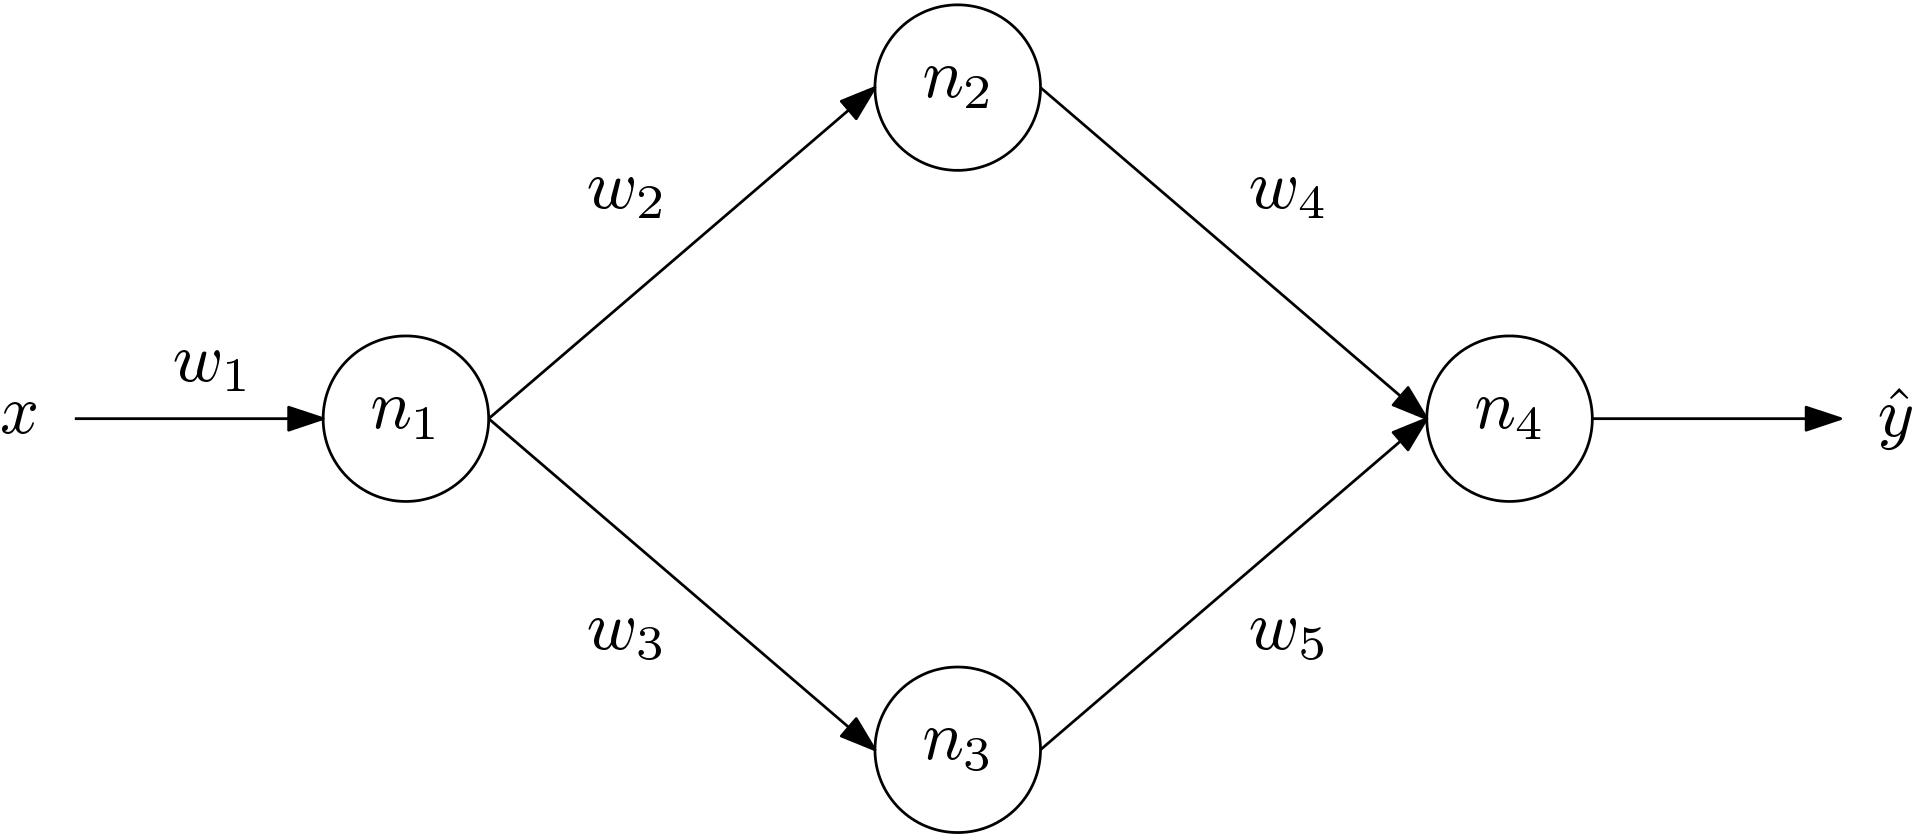
\includegraphics{images/a4_network.png}
\caption{Figure 1}
\end{figure}

It has single input \(x\), and three layers with respectively one, two,
and one neurons. The activation function of the neurons is ReLU.

The parameters \(w_1\), \(w_2\), \(w_3\), \(w_4\), and \(w_5\) (no
biases) are initialized to the following values \(w_1 = 2, w_2 = 1\),
\(w_3 = 2\), \(w_4 = 4\), and \(w_5 = 1\). Implement a single update
step of the gradient descent algorithm by hand. Run the update state for
the data point \((x=2, y=3)\):

The goal is to model the relationship between two continuous variables.
The learning rate is set to \(0.1\)

Provide the solution in the following format:

\begin{itemize}
\tightlist
\item
  A choice for a loss function
\item
  Compute graph for training the neural network
\item
  Partial derivative expression for each of the parameters in the model
\item
  The update expression for each of the parameters for each of the
  data-points
\item
  The final value of all five parameters after the single step in the
  gradient descent algorithm
\end{itemize}

The Python code for simple computational graph nodes, as seen in the
tutorial session, is provided in the cell below (run the cell to load
the code, and again to run the code). Extend the nodes so they can be
used to implement the network described above. Implement the network
with the same initial weights and the correct learning rate, and verify
your hand-made calculations. Add comments to your code or provide a
separate description to explain the changes you have made.

    \begin{Verbatim}[commandchars=\\\{\}]
{\color{incolor}In [{\color{incolor}3}]:} \PY{c+c1}{\PYZsh{} \PYZpc{}load basic\PYZus{}graph.py}
        \PY{l+s+sd}{\PYZsq{}\PYZsq{}\PYZsq{}}
        \PY{l+s+sd}{Implementations of nodes for a computation graph. Each node}
        \PY{l+s+sd}{has a forward pass and a backward pass function, allowing}
        \PY{l+s+sd}{for the evaluation and backpropagation of data.}
        \PY{l+s+sd}{\PYZsq{}\PYZsq{}\PYZsq{}}
        
        \PY{k+kn}{from} \PY{n+nn}{abc} \PY{k}{import} \PY{n}{ABC}\PY{p}{,} \PY{n}{abstractmethod}
        \PY{k+kn}{import} \PY{n+nn}{math}
        \PY{k+kn}{import} \PY{n+nn}{time}
        
        
        \PY{k}{class} \PY{n+nc}{Node}\PY{p}{(}\PY{n+nb}{object}\PY{p}{)}\PY{p}{:}
        
            \PY{k}{def} \PY{n+nf}{\PYZus{}\PYZus{}init\PYZus{}\PYZus{}}\PY{p}{(}\PY{n+nb+bp}{self}\PY{p}{,} \PY{n}{inputs}\PY{p}{)}\PY{p}{:}
                \PY{n+nb+bp}{self}\PY{o}{.}\PY{n}{inputs} \PY{o}{=} \PY{n}{inputs}
        
            \PY{n+nd}{@abstractmethod}
            \PY{k}{def} \PY{n+nf}{forward}\PY{p}{(}\PY{n+nb+bp}{self}\PY{p}{)}\PY{p}{:}
                \PY{l+s+sd}{\PYZsq{}\PYZsq{}\PYZsq{} Feed\PYZhy{}forward the result \PYZsq{}\PYZsq{}\PYZsq{}}
                \PY{k}{raise} \PY{n+ne}{NotImplementedError}\PY{p}{(}\PY{l+s+s2}{\PYZdq{}}\PY{l+s+s2}{Missing forward\PYZhy{}propagation method.}\PY{l+s+s2}{\PYZdq{}}\PY{p}{)}
        
            \PY{n+nd}{@abstractmethod}
            \PY{k}{def} \PY{n+nf}{backward}\PY{p}{(}\PY{n+nb+bp}{self}\PY{p}{,} \PY{n}{d}\PY{p}{)}\PY{p}{:}
                \PY{l+s+sd}{\PYZsq{}\PYZsq{}\PYZsq{} Back\PYZhy{}propagate the error}
        \PY{l+s+sd}{            d is the delta of the subsequent node in the network \PYZsq{}\PYZsq{}\PYZsq{}}
                \PY{k}{raise} \PY{n+ne}{NotImplementedError}\PY{p}{(}\PY{l+s+s2}{\PYZdq{}}\PY{l+s+s2}{Missing back\PYZhy{}propagation method.}\PY{l+s+s2}{\PYZdq{}}\PY{p}{)}
        
        
        \PY{k}{class} \PY{n+nc}{ConstantNode}\PY{p}{(}\PY{n}{Node}\PY{p}{)}\PY{p}{:}
        
            \PY{k}{def} \PY{n+nf}{\PYZus{}\PYZus{}init\PYZus{}\PYZus{}}\PY{p}{(}\PY{n+nb+bp}{self}\PY{p}{,} \PY{n}{value}\PY{p}{)}\PY{p}{:}
                \PY{n+nb+bp}{self}\PY{o}{.}\PY{n}{output} \PY{o}{=} \PY{n}{value}
        
            \PY{k}{def} \PY{n+nf}{forward}\PY{p}{(}\PY{n+nb+bp}{self}\PY{p}{)}\PY{p}{:}
                \PY{k}{return} \PY{n+nb+bp}{self}\PY{o}{.}\PY{n}{output}
        
            \PY{k}{def} \PY{n+nf}{backward}\PY{p}{(}\PY{n+nb+bp}{self}\PY{p}{,} \PY{n}{d}\PY{p}{)}\PY{p}{:}
                \PY{k}{pass}
        
        
        \PY{k}{class} \PY{n+nc}{VariableNode}\PY{p}{(}\PY{n}{Node}\PY{p}{)}\PY{p}{:}
        
            \PY{k}{def} \PY{n+nf}{\PYZus{}\PYZus{}init\PYZus{}\PYZus{}}\PY{p}{(}\PY{n+nb+bp}{self}\PY{p}{,} \PY{n}{value}\PY{p}{)}\PY{p}{:}
                \PY{n+nb+bp}{self}\PY{o}{.}\PY{n}{output} \PY{o}{=} \PY{n}{value}
        
            \PY{k}{def} \PY{n+nf}{forward}\PY{p}{(}\PY{n+nb+bp}{self}\PY{p}{)}\PY{p}{:}
                \PY{k}{return} \PY{n+nb+bp}{self}\PY{o}{.}\PY{n}{output}
        
            \PY{k}{def} \PY{n+nf}{backward}\PY{p}{(}\PY{n+nb+bp}{self}\PY{p}{,} \PY{n}{d}\PY{p}{)}\PY{p}{:}
                \PY{n+nb+bp}{self}\PY{o}{.}\PY{n}{output} \PY{o}{\PYZhy{}}\PY{o}{=} \PY{l+m+mf}{0.1} \PY{o}{*} \PY{n}{d} \PY{c+c1}{\PYZsh{} Gradient Descent}
        
        
        \PY{k}{class} \PY{n+nc}{AdditionNode}\PY{p}{(}\PY{n}{Node}\PY{p}{)}\PY{p}{:}
        
            \PY{k}{def} \PY{n+nf}{forward}\PY{p}{(}\PY{n+nb+bp}{self}\PY{p}{)}\PY{p}{:}
                \PY{n+nb+bp}{self}\PY{o}{.}\PY{n}{output} \PY{o}{=} \PY{n+nb}{sum}\PY{p}{(}\PY{p}{[}\PY{n}{i}\PY{o}{.}\PY{n}{forward}\PY{p}{(}\PY{p}{)} \PY{k}{for} \PY{n}{i} \PY{o+ow}{in} \PY{n+nb+bp}{self}\PY{o}{.}\PY{n}{inputs}\PY{p}{]}\PY{p}{)}
                \PY{k}{return} \PY{n+nb+bp}{self}\PY{o}{.}\PY{n}{output}
        
            \PY{k}{def} \PY{n+nf}{backward}\PY{p}{(}\PY{n+nb+bp}{self}\PY{p}{,} \PY{n}{d}\PY{p}{)}\PY{p}{:}
                \PY{k}{for} \PY{n}{i} \PY{o+ow}{in} \PY{n+nb+bp}{self}\PY{o}{.}\PY{n}{inputs}\PY{p}{:}
                    \PY{n}{i}\PY{o}{.}\PY{n}{backward}\PY{p}{(}\PY{n}{d}\PY{p}{)}
        
        
        \PY{k}{class} \PY{n+nc}{MultiplicationNode}\PY{p}{(}\PY{n}{Node}\PY{p}{)}\PY{p}{:}
        
            \PY{k}{def} \PY{n+nf}{forward}\PY{p}{(}\PY{n+nb+bp}{self}\PY{p}{)}\PY{p}{:}
                \PY{n+nb+bp}{self}\PY{o}{.}\PY{n}{output} \PY{o}{=} \PY{n+nb+bp}{self}\PY{o}{.}\PY{n}{inputs}\PY{p}{[}\PY{l+m+mi}{0}\PY{p}{]}\PY{o}{.}\PY{n}{forward}\PY{p}{(}\PY{p}{)} \PY{o}{*} \PY{n+nb+bp}{self}\PY{o}{.}\PY{n}{inputs}\PY{p}{[}\PY{l+m+mi}{1}\PY{p}{]}\PY{o}{.}\PY{n}{forward}\PY{p}{(}\PY{p}{)}
                \PY{k}{return} \PY{n+nb+bp}{self}\PY{o}{.}\PY{n}{output}
        
            \PY{k}{def} \PY{n+nf}{backward}\PY{p}{(}\PY{n+nb+bp}{self}\PY{p}{,} \PY{n}{d}\PY{p}{)}\PY{p}{:}
                \PY{n+nb+bp}{self}\PY{o}{.}\PY{n}{inputs}\PY{p}{[}\PY{l+m+mi}{0}\PY{p}{]}\PY{o}{.}\PY{n}{backward}\PY{p}{(}\PY{n}{d} \PY{o}{*} \PY{n+nb+bp}{self}\PY{o}{.}\PY{n}{inputs}\PY{p}{[}\PY{l+m+mi}{1}\PY{p}{]}\PY{o}{.}\PY{n}{output}\PY{p}{)}
                \PY{n+nb+bp}{self}\PY{o}{.}\PY{n}{inputs}\PY{p}{[}\PY{l+m+mi}{1}\PY{p}{]}\PY{o}{.}\PY{n}{backward}\PY{p}{(}\PY{n}{d} \PY{o}{*} \PY{n+nb+bp}{self}\PY{o}{.}\PY{n}{inputs}\PY{p}{[}\PY{l+m+mi}{0}\PY{p}{]}\PY{o}{.}\PY{n}{output}\PY{p}{)}
        
        
        \PY{k}{class} \PY{n+nc}{MSENode}\PY{p}{(}\PY{n}{Node}\PY{p}{)}\PY{p}{:}
        
            \PY{k}{def} \PY{n+nf}{forward}\PY{p}{(}\PY{n+nb+bp}{self}\PY{p}{)}\PY{p}{:}
                \PY{n+nb+bp}{self}\PY{o}{.}\PY{n}{output} \PY{o}{=} \PY{l+m+mf}{0.5} \PY{o}{*} \PY{p}{(}
                    \PY{n+nb+bp}{self}\PY{o}{.}\PY{n}{inputs}\PY{p}{[}\PY{l+m+mi}{0}\PY{p}{]}\PY{o}{.}\PY{n}{forward}\PY{p}{(}\PY{p}{)} \PY{o}{\PYZhy{}} \PY{n+nb+bp}{self}\PY{o}{.}\PY{n}{inputs}\PY{p}{[}\PY{l+m+mi}{1}\PY{p}{]}\PY{o}{.}\PY{n}{forward}\PY{p}{(}\PY{p}{)}\PY{p}{)}\PY{o}{*}\PY{o}{*}\PY{l+m+mi}{2}
                \PY{k}{return} \PY{n+nb+bp}{self}\PY{o}{.}\PY{n}{output}
        
            \PY{k}{def} \PY{n+nf}{backward}\PY{p}{(}\PY{n+nb+bp}{self}\PY{p}{,} \PY{n}{d}\PY{p}{)}\PY{p}{:}
                \PY{n+nb+bp}{self}\PY{o}{.}\PY{n}{inputs}\PY{p}{[}\PY{l+m+mi}{0}\PY{p}{]}\PY{o}{.}\PY{n}{backward}\PY{p}{(}\PY{n}{d} \PY{o}{*} \PY{p}{(}\PY{n+nb+bp}{self}\PY{o}{.}\PY{n}{inputs}\PY{p}{[}\PY{l+m+mi}{0}\PY{p}{]}\PY{o}{.}\PY{n}{output} \PY{o}{\PYZhy{}} \PY{n+nb+bp}{self}\PY{o}{.}\PY{n}{inputs}\PY{p}{[}\PY{l+m+mi}{1}\PY{p}{]}\PY{o}{.}\PY{n}{output}\PY{p}{)}\PY{p}{)}
                \PY{n+nb+bp}{self}\PY{o}{.}\PY{n}{inputs}\PY{p}{[}\PY{l+m+mi}{1}\PY{p}{]}\PY{o}{.}\PY{n}{backward}\PY{p}{(}\PY{n}{d} \PY{o}{*} \PY{p}{(}\PY{n+nb+bp}{self}\PY{o}{.}\PY{n}{inputs}\PY{p}{[}\PY{l+m+mi}{1}\PY{p}{]}\PY{o}{.}\PY{n}{output} \PY{o}{\PYZhy{}} \PY{n+nb+bp}{self}\PY{o}{.}\PY{n}{inputs}\PY{p}{[}\PY{l+m+mi}{0}\PY{p}{]}\PY{o}{.}\PY{n}{output}\PY{p}{)}\PY{p}{)}
        
        
        \PY{k}{class} \PY{n+nc}{SigmoidNode}\PY{p}{(}\PY{n}{Node}\PY{p}{)}\PY{p}{:}
        
            \PY{k}{def} \PY{n+nf}{forward}\PY{p}{(}\PY{n+nb+bp}{self}\PY{p}{)}\PY{p}{:}
                \PY{n+nb+bp}{self}\PY{o}{.}\PY{n}{output} \PY{o}{=} \PY{l+m+mf}{1.0} \PY{o}{/} \PY{p}{(}\PY{l+m+mf}{1.0} \PY{o}{+} \PY{n}{math}\PY{o}{.}\PY{n}{exp}\PY{p}{(}\PY{o}{\PYZhy{}}\PY{n+nb+bp}{self}\PY{o}{.}\PY{n}{inputs}\PY{p}{[}\PY{l+m+mi}{0}\PY{p}{]}\PY{o}{.}\PY{n}{forward}\PY{p}{(}\PY{p}{)}\PY{p}{)}\PY{p}{)}
                \PY{k}{return} \PY{n+nb+bp}{self}\PY{o}{.}\PY{n}{output}
        
            \PY{k}{def} \PY{n+nf}{backward}\PY{p}{(}\PY{n+nb+bp}{self}\PY{p}{,} \PY{n}{d}\PY{p}{)}\PY{p}{:}
                \PY{n+nb+bp}{self}\PY{o}{.}\PY{n}{inputs}\PY{p}{[}\PY{l+m+mi}{0}\PY{p}{]}\PY{o}{.}\PY{n}{backward}\PY{p}{(}\PY{n}{d} \PY{o}{*} \PY{n+nb+bp}{self}\PY{o}{.}\PY{n}{output} \PY{o}{*} \PY{p}{(}\PY{l+m+mf}{1.0} \PY{o}{\PYZhy{}} \PY{n+nb+bp}{self}\PY{o}{.}\PY{n}{output}\PY{p}{)}\PY{p}{)}
        
        \PY{k}{class} \PY{n+nc}{ReLUNode}\PY{p}{(}\PY{n+nb}{object}\PY{p}{)}\PY{p}{:}
        
            \PY{k}{def} \PY{n+nf}{forward}\PY{p}{(}\PY{n+nb+bp}{self}\PY{p}{)}\PY{p}{:}
                \PY{k}{raise} \PY{n+ne}{NotImplementedError}\PY{p}{(}\PY{l+s+s2}{\PYZdq{}}\PY{l+s+s2}{Forward pass for ReLU activation node has not been implemented yet.}\PY{l+s+s2}{\PYZdq{}}\PY{p}{)}
        
            \PY{k}{def} \PY{n+nf}{backward}\PY{p}{(}\PY{n+nb+bp}{self}\PY{p}{,} \PY{n}{d}\PY{p}{)}\PY{p}{:}
                \PY{k}{raise} \PY{n+ne}{NotImplementedError}\PY{p}{(}\PY{l+s+s2}{\PYZdq{}}\PY{l+s+s2}{Backward pass for ReLU activation node has not been implemented yet.}\PY{l+s+s2}{\PYZdq{}}\PY{p}{)}
        
        \PY{k}{class} \PY{n+nc}{TanhNode}\PY{p}{(}\PY{n+nb}{object}\PY{p}{)}\PY{p}{:}
        
            \PY{k}{def} \PY{n+nf}{forward}\PY{p}{(}\PY{n+nb+bp}{self}\PY{p}{)}\PY{p}{:}
                \PY{k}{raise} \PY{n+ne}{NotImplementedError}\PY{p}{(}\PY{l+s+s2}{\PYZdq{}}\PY{l+s+s2}{Forward pass for tanh activation node has not been implemented yet.}\PY{l+s+s2}{\PYZdq{}}\PY{p}{)}
        
            \PY{k}{def} \PY{n+nf}{backward}\PY{p}{(}\PY{n+nb+bp}{self}\PY{p}{,} \PY{n}{d}\PY{p}{)}\PY{p}{:}
                \PY{k}{raise} \PY{n+ne}{NotImplementedError}\PY{p}{(}\PY{l+s+s2}{\PYZdq{}}\PY{l+s+s2}{Backward pass for tanh activation node has not been implemented yet.}\PY{l+s+s2}{\PYZdq{}}\PY{p}{)}
        
        \PY{c+c1}{\PYZsh{} Example graph as shown in MLP lecture slides}
        \PY{k}{class} \PY{n+nc}{SampleGraph}\PY{p}{(}\PY{n+nb}{object}\PY{p}{)}\PY{p}{:}
        
            \PY{k}{def} \PY{n+nf}{\PYZus{}\PYZus{}init\PYZus{}\PYZus{}}\PY{p}{(}\PY{n+nb+bp}{self}\PY{p}{,} \PY{n}{x}\PY{p}{,} \PY{n}{y}\PY{p}{,} \PY{n}{w}\PY{p}{,} \PY{n}{b}\PY{p}{)}\PY{p}{:}
                \PY{l+s+sd}{\PYZsq{}\PYZsq{}\PYZsq{} x: input}
        \PY{l+s+sd}{            y: expected output}
        \PY{l+s+sd}{            w: initial weight}
        \PY{l+s+sd}{            b: initial bias \PYZsq{}\PYZsq{}\PYZsq{}}
                \PY{n+nb+bp}{self}\PY{o}{.}\PY{n}{w} \PY{o}{=} \PY{n}{VariableNode}\PY{p}{(}\PY{n}{w}\PY{p}{)}
                \PY{n+nb+bp}{self}\PY{o}{.}\PY{n}{b} \PY{o}{=} \PY{n}{VariableNode}\PY{p}{(}\PY{n}{b}\PY{p}{)}
                \PY{n+nb+bp}{self}\PY{o}{.}\PY{n}{graph} \PY{o}{=} \PY{n}{MSENode}\PY{p}{(}\PY{p}{[}
                    \PY{n}{AdditionNode}\PY{p}{(}\PY{p}{[}
                        \PY{n}{MultiplicationNode}\PY{p}{(}\PY{p}{[}
                            \PY{n}{ConstantNode}\PY{p}{(}\PY{n}{x}\PY{p}{)}\PY{p}{,}
                            \PY{n+nb+bp}{self}\PY{o}{.}\PY{n}{w}
                        \PY{p}{]}\PY{p}{)}\PY{p}{,}
                        \PY{n}{MultiplicationNode}\PY{p}{(}\PY{p}{[}
                            \PY{n+nb+bp}{self}\PY{o}{.}\PY{n}{b}\PY{p}{,}
                            \PY{n}{ConstantNode}\PY{p}{(}\PY{l+m+mi}{1}\PY{p}{)}
                        \PY{p}{]}\PY{p}{)}
                    \PY{p}{]}\PY{p}{)}\PY{p}{,}
                    \PY{n}{ConstantNode}\PY{p}{(}\PY{n}{y}\PY{p}{)}
                \PY{p}{]}\PY{p}{)}
        
            \PY{k}{def} \PY{n+nf}{forward}\PY{p}{(}\PY{n+nb+bp}{self}\PY{p}{)}\PY{p}{:}
                \PY{k}{return} \PY{n+nb+bp}{self}\PY{o}{.}\PY{n}{graph}\PY{o}{.}\PY{n}{forward}\PY{p}{(}\PY{p}{)}
        
            \PY{k}{def} \PY{n+nf}{backward}\PY{p}{(}\PY{n+nb+bp}{self}\PY{p}{,} \PY{n}{d}\PY{p}{)}\PY{p}{:}
                \PY{n+nb+bp}{self}\PY{o}{.}\PY{n}{graph}\PY{o}{.}\PY{n}{backward}\PY{p}{(}\PY{n}{d}\PY{p}{)}
        
        
        \PY{k}{class} \PY{n+nc}{Neuron}\PY{p}{(}\PY{n}{Node}\PY{p}{)}\PY{p}{:}
        
            \PY{k}{def} \PY{n+nf}{\PYZus{}\PYZus{}init\PYZus{}\PYZus{}}\PY{p}{(}\PY{n+nb+bp}{self}\PY{p}{,} \PY{n}{inputs}\PY{p}{,} \PY{n}{weights}\PY{p}{,} \PY{n}{activation}\PY{p}{)}\PY{p}{:}
                \PY{l+s+sd}{\PYZsq{}\PYZsq{}\PYZsq{} weights: list of initial weights, same length as inputs \PYZsq{}\PYZsq{}\PYZsq{}}
                \PY{n+nb+bp}{self}\PY{o}{.}\PY{n}{inputs} \PY{o}{=} \PY{n}{inputs}
                \PY{c+c1}{\PYZsh{} Initialize a weight for each input}
                \PY{n+nb+bp}{self}\PY{o}{.}\PY{n}{weights} \PY{o}{=} \PY{p}{[}\PY{n}{VariableNode}\PY{p}{(}\PY{n}{weight}\PY{p}{)} \PY{k}{for} \PY{n}{weight} \PY{o+ow}{in} \PY{n}{weights}\PY{p}{]}
                \PY{c+c1}{\PYZsh{} Neurons normally have a bias, ignore for this assignment}
                \PY{c+c1}{\PYZsh{}self.bias = VariableNode(bias, \PYZdq{}b\PYZdq{})}
        
                \PY{c+c1}{\PYZsh{} Multiplication node for each pair of inputs and weights}
                \PY{n}{mults} \PY{o}{=} \PY{p}{[}\PY{n}{MultiplicationNode}\PY{p}{(}\PY{p}{[}\PY{n}{i}\PY{p}{,} \PY{n}{w}\PY{p}{]}\PY{p}{)} \PY{k}{for} \PY{n}{i}\PY{p}{,} \PY{n}{w}\PY{p}{,} \PY{o+ow}{in} \PY{n+nb}{zip}\PY{p}{(}\PY{n+nb+bp}{self}\PY{o}{.}\PY{n}{inputs}\PY{p}{,} \PY{n+nb+bp}{self}\PY{o}{.}\PY{n}{weights}\PY{p}{)}\PY{p}{]}
                \PY{c+c1}{\PYZsh{} Neurons normally have a bias, ignore for this assignment}
                \PY{c+c1}{\PYZsh{}mults.append(MultiplicationNode([self.bias, ConstantNode(1)]))}
        
                \PY{c+c1}{\PYZsh{} Sum all multiplication results}
                \PY{n}{added} \PY{o}{=} \PY{n}{AdditionNode}\PY{p}{(}\PY{n}{mults}\PY{p}{)}
        
                \PY{c+c1}{\PYZsh{} Apply activation function}
                \PY{k}{if} \PY{n}{activation} \PY{o}{==} \PY{l+s+s1}{\PYZsq{}}\PY{l+s+s1}{sigmoid}\PY{l+s+s1}{\PYZsq{}}\PY{p}{:}
                    \PY{n+nb+bp}{self}\PY{o}{.}\PY{n}{graph} \PY{o}{=} \PY{n}{SigmoidNode}\PY{p}{(}\PY{p}{[}\PY{n}{added}\PY{p}{]}\PY{p}{)}
                \PY{k}{elif} \PY{n}{activation} \PY{o}{==} \PY{l+s+s1}{\PYZsq{}}\PY{l+s+s1}{relu}\PY{l+s+s1}{\PYZsq{}}\PY{p}{:}
                    \PY{n+nb+bp}{self}\PY{o}{.}\PY{n}{graph} \PY{o}{=} \PY{n}{ReLUNode}\PY{p}{(}\PY{p}{[}\PY{n}{added}\PY{p}{]}\PY{p}{)}
                \PY{k}{elif} \PY{n}{activation} \PY{o}{==} \PY{l+s+s1}{\PYZsq{}}\PY{l+s+s1}{tanh}\PY{l+s+s1}{\PYZsq{}}\PY{p}{:}
                    \PY{n+nb+bp}{self}\PY{o}{.}\PY{n}{graph} \PY{o}{=} \PY{n}{TanhNode}\PY{p}{(}\PY{p}{[}\PY{n}{added}\PY{p}{]}\PY{p}{)}
                \PY{k}{else}\PY{p}{:}
                    \PY{k}{raise} \PY{n+ne}{ValueError}\PY{p}{(}\PY{l+s+s2}{\PYZdq{}}\PY{l+s+s2}{Unknown activation function.}\PY{l+s+s2}{\PYZdq{}}\PY{p}{)}
        
            \PY{k}{def} \PY{n+nf}{forward}\PY{p}{(}\PY{n+nb+bp}{self}\PY{p}{)}\PY{p}{:}
                \PY{k}{return} \PY{n+nb+bp}{self}\PY{o}{.}\PY{n}{graph}\PY{o}{.}\PY{n}{forward}\PY{p}{(}\PY{p}{)}
        
            \PY{k}{def} \PY{n+nf}{backward}\PY{p}{(}\PY{n+nb+bp}{self}\PY{p}{,} \PY{n}{d}\PY{p}{)}\PY{p}{:}
                \PY{n+nb+bp}{self}\PY{o}{.}\PY{n}{graph}\PY{o}{.}\PY{n}{backward}\PY{p}{(}\PY{n}{d}\PY{p}{)}
        
            \PY{k}{def} \PY{n+nf}{set\PYZus{}weights}\PY{p}{(}\PY{n+nb+bp}{self}\PY{p}{,} \PY{n}{new\PYZus{}weights}\PY{p}{)}\PY{p}{:}
                \PY{k}{for} \PY{n}{i} \PY{o+ow}{in} \PY{n+nb}{len}\PY{p}{(}\PY{n}{new\PYZus{}weights}\PY{p}{)}\PY{p}{:}
                    \PY{n+nb+bp}{self}\PY{o}{.}\PY{n}{weights}\PY{p}{[}\PY{n}{i}\PY{p}{]}\PY{o}{.}\PY{n}{output} \PY{o}{=} \PY{n}{new\PYZus{}weights}\PY{p}{[}\PY{n}{i}\PY{p}{]}
        
            \PY{k}{def} \PY{n+nf}{get\PYZus{}weights}\PY{p}{(}\PY{n+nb+bp}{self}\PY{p}{)}\PY{p}{:}
                \PY{k}{return} \PY{p}{[}\PY{n}{weight}\PY{o}{.}\PY{n}{output} \PY{k}{for} \PY{n}{weight} \PY{o+ow}{in} \PY{n+nb+bp}{self}\PY{o}{.}\PY{n}{weights}\PY{p}{]}
        
        \PY{k}{if} \PY{n+nv+vm}{\PYZus{}\PYZus{}name\PYZus{}\PYZus{}} \PY{o}{==} \PY{l+s+s1}{\PYZsq{}}\PY{l+s+s1}{\PYZus{}\PYZus{}main\PYZus{}\PYZus{}}\PY{l+s+s1}{\PYZsq{}}\PY{p}{:}
            \PY{n+nb}{print}\PY{p}{(}\PY{l+s+s2}{\PYZdq{}}\PY{l+s+s2}{Loaded simple graph nodes}\PY{l+s+s2}{\PYZdq{}}\PY{p}{)}
        
            \PY{c+c1}{\PYZsh{} Example network}
            \PY{c+c1}{\PYZsh{}sg = SampleGraph(2, 2, 2, 1)}
            \PY{c+c1}{\PYZsh{}prediction = sg.forward()}
            \PY{c+c1}{\PYZsh{}print(\PYZdq{}Initial prediction is\PYZdq{}, prediction)}
            \PY{c+c1}{\PYZsh{}sg.backward(1)}
            \PY{c+c1}{\PYZsh{}print(\PYZdq{}w has new value\PYZdq{}, sg.w.output)}
            \PY{c+c1}{\PYZsh{}print(\PYZdq{}b has new value\PYZdq{}, sg.b.output)}
        
            \PY{c+c1}{\PYZsh{} Run your network here}
        \PY{k}{class} \PY{n+nc}{MyGraph}\PY{p}{(}\PY{n+nb}{object}\PY{p}{)}\PY{p}{:}
        
            \PY{k}{def} \PY{n+nf}{\PYZus{}\PYZus{}init\PYZus{}\PYZus{}}\PY{p}{(}\PY{n+nb+bp}{self}\PY{p}{,} \PY{n}{x}\PY{p}{,} \PY{n}{y}\PY{p}{,} \PY{n}{weigths}\PY{p}{)}\PY{p}{:}
                \PY{l+s+sd}{\PYZsq{}\PYZsq{}\PYZsq{} x: input}
        \PY{l+s+sd}{            y: expected output}
        \PY{l+s+sd}{            w: initial weight}
        \PY{l+s+sd}{            b: initial bias \PYZsq{}\PYZsq{}\PYZsq{}}
                               
                \PY{n+nb+bp}{self}\PY{o}{.}\PY{n}{weights} \PY{o}{=} \PY{p}{[}\PY{n}{VariableNode}\PY{p}{(}\PY{n}{weight}\PY{p}{)} \PY{k}{for} \PY{n}{weight} \PY{o+ow}{in} \PY{n}{weigths}\PY{p}{]}
                
                \PY{n+nb+bp}{self}\PY{o}{.}\PY{n}{z1} \PY{o}{=} \PY{n}{MultiplicationNode}\PY{p}{(}\PY{p}{[}\PY{n}{ConstantNode}\PY{p}{(}\PY{n}{x}\PY{p}{)}\PY{p}{,}\PY{n+nb+bp}{self}\PY{o}{.}\PY{n}{weights}\PY{p}{[}\PY{l+m+mi}{0}\PY{p}{]}\PY{p}{]}\PY{p}{)}
                \PY{n+nb+bp}{self}\PY{o}{.}\PY{n}{n1} \PY{o}{=} \PY{n}{SigmoidNode}\PY{p}{(}\PY{p}{[}\PY{n+nb+bp}{self}\PY{o}{.}\PY{n}{z1}\PY{p}{]}\PY{p}{)}
                \PY{n+nb+bp}{self}\PY{o}{.}\PY{n}{z2} \PY{o}{=} \PY{n}{MultiplicationNode}\PY{p}{(}\PY{p}{[}\PY{n+nb+bp}{self}\PY{o}{.}\PY{n}{n1}\PY{p}{,} \PY{n+nb+bp}{self}\PY{o}{.}\PY{n}{weights}\PY{p}{[}\PY{l+m+mi}{1}\PY{p}{]}\PY{p}{]}\PY{p}{)}
                \PY{n+nb+bp}{self}\PY{o}{.}\PY{n}{n2} \PY{o}{=} \PY{n}{SigmoidNode}\PY{p}{(}\PY{p}{[}\PY{n+nb+bp}{self}\PY{o}{.}\PY{n}{z2}\PY{p}{]}\PY{p}{)}
                \PY{n+nb+bp}{self}\PY{o}{.}\PY{n}{z3} \PY{o}{=} \PY{n}{MultiplicationNode}\PY{p}{(}\PY{p}{[}\PY{n+nb+bp}{self}\PY{o}{.}\PY{n}{n1}\PY{p}{,} \PY{n+nb+bp}{self}\PY{o}{.}\PY{n}{weights}\PY{p}{[}\PY{l+m+mi}{2}\PY{p}{]}\PY{p}{]}\PY{p}{)}
                \PY{n+nb+bp}{self}\PY{o}{.}\PY{n}{n3} \PY{o}{=} \PY{n}{SigmoidNode}\PY{p}{(}\PY{p}{[}\PY{n+nb+bp}{self}\PY{o}{.}\PY{n}{z3}\PY{p}{]}\PY{p}{)}
                \PY{n+nb+bp}{self}\PY{o}{.}\PY{n}{z4} \PY{o}{=} \PY{n}{AdditionNode}\PY{p}{(}\PY{p}{[}\PY{n}{MultiplicationNode}\PY{p}{(}\PY{p}{[}
                                     \PY{n+nb+bp}{self}\PY{o}{.}\PY{n}{n2}\PY{p}{,}
                                     \PY{n+nb+bp}{self}\PY{o}{.}\PY{n}{weights}\PY{p}{[}\PY{l+m+mi}{3}\PY{p}{]}\PY{p}{]}\PY{p}{)}\PY{p}{,}
                                     \PY{n}{MultiplicationNode}\PY{p}{(}\PY{p}{[}
                                     \PY{n+nb+bp}{self}\PY{o}{.}\PY{n}{n3}\PY{p}{,}
                                     \PY{n+nb+bp}{self}\PY{o}{.}\PY{n}{weights}\PY{p}{[}\PY{l+m+mi}{4}\PY{p}{]}\PY{p}{]}\PY{p}{)}\PY{p}{]}\PY{p}{)}
                \PY{n+nb+bp}{self}\PY{o}{.}\PY{n}{n4} \PY{o}{=} \PY{n}{SigmoidNode}\PY{p}{(}\PY{p}{[}\PY{n+nb+bp}{self}\PY{o}{.}\PY{n}{z4}\PY{p}{]}\PY{p}{)}
                \PY{n+nb+bp}{self}\PY{o}{.}\PY{n}{graph} \PY{o}{=} \PY{n}{MSENode}\PY{p}{(}\PY{p}{[}\PY{n+nb+bp}{self}\PY{o}{.}\PY{n}{n4}\PY{p}{,}\PY{n}{ConstantNode}\PY{p}{(}\PY{n}{y}\PY{p}{)}\PY{p}{]}\PY{p}{)}
        
            \PY{k}{def} \PY{n+nf}{forward}\PY{p}{(}\PY{n+nb+bp}{self}\PY{p}{)}\PY{p}{:}
                \PY{k}{return} \PY{n+nb+bp}{self}\PY{o}{.}\PY{n}{graph}\PY{o}{.}\PY{n}{forward}\PY{p}{(}\PY{p}{)}
        
            \PY{k}{def} \PY{n+nf}{backward}\PY{p}{(}\PY{n+nb+bp}{self}\PY{p}{,} \PY{n}{d}\PY{p}{)}\PY{p}{:}
                \PY{n+nb+bp}{self}\PY{o}{.}\PY{n}{graph}\PY{o}{.}\PY{n}{backward}\PY{p}{(}\PY{n}{d}\PY{p}{)}
            \PY{k}{def} \PY{n+nf}{set\PYZus{}weights}\PY{p}{(}\PY{n+nb+bp}{self}\PY{p}{,} \PY{n}{new\PYZus{}weights}\PY{p}{)}\PY{p}{:}
                \PY{k}{for} \PY{n}{i} \PY{o+ow}{in} \PY{n+nb}{len}\PY{p}{(}\PY{n}{new\PYZus{}weights}\PY{p}{)}\PY{p}{:}
                    \PY{n+nb+bp}{self}\PY{o}{.}\PY{n}{weights}\PY{p}{[}\PY{n}{i}\PY{p}{]}\PY{o}{.}\PY{n}{output} \PY{o}{=} \PY{n}{new\PYZus{}weights}\PY{p}{[}\PY{n}{i}\PY{p}{]}
        
            \PY{k}{def} \PY{n+nf}{get\PYZus{}weights}\PY{p}{(}\PY{n+nb+bp}{self}\PY{p}{)}\PY{p}{:}
                \PY{k}{return} \PY{p}{[}\PY{n}{weight}\PY{o}{.}\PY{n}{output} \PY{k}{for} \PY{n}{weight} \PY{o+ow}{in} \PY{n+nb+bp}{self}\PY{o}{.}\PY{n}{weights}\PY{p}{]}
        
        \PY{n}{x}\PY{o}{=}\PY{l+m+mi}{2}
        \PY{n}{y}\PY{o}{=}\PY{l+m+mi}{3}
        \PY{n}{w1}\PY{o}{=}\PY{l+m+mi}{2}
        \PY{n}{w2}\PY{o}{=}\PY{l+m+mi}{1}
        \PY{n}{w3}\PY{o}{=}\PY{l+m+mi}{2}
        \PY{n}{w4}\PY{o}{=}\PY{l+m+mi}{4}
        \PY{n}{w5}\PY{o}{=}\PY{l+m+mi}{1}
        
        
        \PY{n}{sg} \PY{o}{=} \PY{n}{MyGraph}\PY{p}{(}\PY{n}{x}\PY{p}{,} \PY{n}{y}\PY{p}{,}\PY{p}{[}\PY{n}{w1}\PY{p}{,}\PY{n}{w2}\PY{p}{,}\PY{n}{w3}\PY{p}{,}\PY{n}{w4}\PY{p}{,}\PY{n}{w5}\PY{p}{]}\PY{p}{)}
        
        \PY{n}{Error1} \PY{o}{=} \PY{n}{sg}\PY{o}{.}\PY{n}{forward}\PY{p}{(}\PY{p}{)}
        
        \PY{n+nb}{print}\PY{p}{(}\PY{n}{sg}\PY{o}{.}\PY{n}{z1}\PY{o}{.}\PY{n}{output}\PY{p}{)}
        \PY{n+nb}{print}\PY{p}{(}\PY{n}{sg}\PY{o}{.}\PY{n}{n1}\PY{o}{.}\PY{n}{output}\PY{p}{)}
        \PY{n+nb}{print}\PY{p}{(}\PY{n}{sg}\PY{o}{.}\PY{n}{n2}\PY{o}{.}\PY{n}{output}\PY{p}{)}
        \PY{n+nb}{print}\PY{p}{(}\PY{n}{sg}\PY{o}{.}\PY{n}{n3}\PY{o}{.}\PY{n}{output}\PY{p}{)}
        \PY{n+nb}{print}\PY{p}{(}\PY{n}{sg}\PY{o}{.}\PY{n}{n4}\PY{o}{.}\PY{n}{output}\PY{p}{)}
        \PY{n+nb}{print}\PY{p}{(}\PY{l+s+s2}{\PYZdq{}}\PY{l+s+s2}{Graph}\PY{l+s+s2}{\PYZdq{}}\PY{p}{,}\PY{n}{sg}\PY{o}{.}\PY{n}{graph}\PY{o}{.}\PY{n}{output}\PY{p}{)}
        
        \PY{n}{sg}\PY{o}{.}\PY{n}{backward}\PY{p}{(}\PY{n}{sg}\PY{o}{.}\PY{n}{n4}\PY{o}{.}\PY{n}{output}\PY{p}{)}
        
        \PY{n}{new\PYZus{}weights}\PY{o}{=}\PY{n}{sg}\PY{o}{.}\PY{n}{get\PYZus{}weights}\PY{p}{(}\PY{p}{)}
        \PY{n+nb}{print}\PY{p}{(}\PY{l+s+s2}{\PYZdq{}}\PY{l+s+s2}{w has new value}\PY{l+s+s2}{\PYZdq{}}\PY{p}{,} \PY{n}{np}\PY{o}{.}\PY{n}{transpose}\PY{p}{(}\PY{n}{new\PYZus{}weights}\PY{p}{)}\PY{p}{)}
\end{Verbatim}


\begin{Verbatim}[commandchars=\\\{\}]
{\color{outcolor}Out[{\color{outcolor}3}]:} '\textbackslash{}nImplementations of nodes for a computation graph. Each node\textbackslash{}nhas a forward pass and a backward pass function, allowing\textbackslash{}nfor the evaluation and backpropagation of data.\textbackslash{}n'
\end{Verbatim}
            
    \begin{Verbatim}[commandchars=\\\{\}]
Loaded simple graph nodes
4
0.9820137900379085
0.7275076135036415
0.8769681683739503
0.9778387307456168
Graph 2.0445680994362494
w has new value [2.    1.003 2.    4.003 1.004]

    \end{Verbatim}

    \subsection{Training Deep Models (3
points)}\label{training-deep-models-3-points}

The model in the example code below performs poorly as its depth
increases. Train this model on the MNIST digit detection task.

Examine its training performance by gradually increasing its depth: -
Set the depth to 1 hidden layer - Set the depth to 2 hidden layers - Set
the depth to 3 hidden layers

Modify the model such that you improve its performance when its depth
increases. Train the new model again for the different depths: - Set the
depth to 1 hidden layer - Set the depth to 2 hidden layers - Set the
depth to 3 hidden layers

Submit an explanation for the limitation of the original model. Explain
your modification. Submit your code and 6 plots (can be overlaid) for
the training performance of both models with different depths.

    \begin{Verbatim}[commandchars=\\\{\}]
{\color{incolor}In [{\color{incolor}27}]:} \PY{c+c1}{\PYZsh{} (You don\PYZsq{}t need to change this part of the code)}
         \PY{k+kn}{from} \PY{n+nn}{\PYZus{}\PYZus{}future\PYZus{}\PYZus{}} \PY{k}{import} \PY{n}{print\PYZus{}function}
         \PY{k+kn}{import} \PY{n+nn}{numpy} \PY{k}{as} \PY{n+nn}{np}
         \PY{n}{np}\PY{o}{.}\PY{n}{random}\PY{o}{.}\PY{n}{seed}\PY{p}{(}\PY{l+m+mi}{1234}\PY{p}{)}
         
         \PY{k+kn}{from} \PY{n+nn}{keras}\PY{n+nn}{.}\PY{n+nn}{datasets} \PY{k}{import} \PY{n}{mnist}
         \PY{k+kn}{from} \PY{n+nn}{keras}\PY{n+nn}{.}\PY{n+nn}{models} \PY{k}{import} \PY{n}{Sequential}
         \PY{k+kn}{from} \PY{n+nn}{keras}\PY{n+nn}{.}\PY{n+nn}{layers}\PY{n+nn}{.}\PY{n+nn}{core} \PY{k}{import} \PY{n}{Dense}\PY{p}{,} \PY{n}{Dropout}\PY{p}{,} \PY{n}{Activation}
         \PY{k+kn}{from} \PY{n+nn}{keras}\PY{n+nn}{.}\PY{n+nn}{optimizers} \PY{k}{import} \PY{n}{SGD}
         \PY{k+kn}{from} \PY{n+nn}{keras}\PY{n+nn}{.}\PY{n+nn}{utils} \PY{k}{import} \PY{n}{np\PYZus{}utils}
         \PY{k+kn}{from} \PY{n+nn}{keras}\PY{n+nn}{.}\PY{n+nn}{layers} \PY{k}{import} \PY{n}{Conv2D}\PY{p}{,} \PY{n}{MaxPooling2D}\PY{p}{,} \PY{n}{Conv1D}\PY{p}{,} \PY{n}{Dense}\PY{p}{,} \PY{n}{TimeDistributed}\PY{p}{,} \PY{n}{Activation}
         
         \PY{k+kn}{import} \PY{n+nn}{matplotlib}\PY{n+nn}{.}\PY{n+nn}{pyplot} \PY{k}{as} \PY{n+nn}{plt}
         
         \PY{n}{batch\PYZus{}size} \PY{o}{=} \PY{l+m+mi}{128}
         \PY{n}{nb\PYZus{}classes} \PY{o}{=} \PY{l+m+mi}{10}
         \PY{n}{nb\PYZus{}epoch} \PY{o}{=} \PY{l+m+mi}{10}
\end{Verbatim}


    \begin{Verbatim}[commandchars=\\\{\}]
{\color{incolor}In [{\color{incolor}28}]:} \PY{c+c1}{\PYZsh{} (You don\PYZsq{}t need to change this part of the code)}
         \PY{c+c1}{\PYZsh{} the data, shuffled and split between train and test sets}
         \PY{p}{(}\PY{n}{X\PYZus{}train}\PY{p}{,} \PY{n}{y\PYZus{}train}\PY{p}{)}\PY{p}{,} \PY{p}{(}\PY{n}{X\PYZus{}test}\PY{p}{,} \PY{n}{y\PYZus{}test}\PY{p}{)} \PY{o}{=} \PY{n}{mnist}\PY{o}{.}\PY{n}{load\PYZus{}data}\PY{p}{(}\PY{p}{)}
         
         \PY{n}{X\PYZus{}train} \PY{o}{=} \PY{n}{X\PYZus{}train}\PY{o}{.}\PY{n}{reshape}\PY{p}{(}\PY{l+m+mi}{60000}\PY{p}{,} \PY{l+m+mi}{784}\PY{p}{)}
         \PY{n}{X\PYZus{}test} \PY{o}{=} \PY{n}{X\PYZus{}test}\PY{o}{.}\PY{n}{reshape}\PY{p}{(}\PY{l+m+mi}{10000}\PY{p}{,} \PY{l+m+mi}{784}\PY{p}{)}
         
         \PY{n}{X\PYZus{}train} \PY{o}{=} \PY{n}{X\PYZus{}train}\PY{o}{.}\PY{n}{astype}\PY{p}{(}\PY{l+s+s1}{\PYZsq{}}\PY{l+s+s1}{float32}\PY{l+s+s1}{\PYZsq{}}\PY{p}{)}
         \PY{n}{X\PYZus{}test} \PY{o}{=} \PY{n}{X\PYZus{}test}\PY{o}{.}\PY{n}{astype}\PY{p}{(}\PY{l+s+s1}{\PYZsq{}}\PY{l+s+s1}{float32}\PY{l+s+s1}{\PYZsq{}}\PY{p}{)}
         \PY{n}{X\PYZus{}train} \PY{o}{/}\PY{o}{=} \PY{l+m+mi}{255}
         \PY{n}{X\PYZus{}test} \PY{o}{/}\PY{o}{=} \PY{l+m+mi}{255}
         \PY{n+nb}{print}\PY{p}{(}\PY{n}{X\PYZus{}train}\PY{o}{.}\PY{n}{shape}\PY{p}{[}\PY{l+m+mi}{0}\PY{p}{]}\PY{p}{,} \PY{l+s+s1}{\PYZsq{}}\PY{l+s+s1}{train samples}\PY{l+s+s1}{\PYZsq{}}\PY{p}{)}
         \PY{n+nb}{print}\PY{p}{(}\PY{n}{X\PYZus{}test}\PY{o}{.}\PY{n}{shape}\PY{p}{[}\PY{l+m+mi}{0}\PY{p}{]}\PY{p}{,} \PY{l+s+s1}{\PYZsq{}}\PY{l+s+s1}{test samples}\PY{l+s+s1}{\PYZsq{}}\PY{p}{)}
         
         \PY{c+c1}{\PYZsh{} convert class vectors to binary class matrices}
         \PY{n}{Y\PYZus{}train} \PY{o}{=} \PY{n}{np\PYZus{}utils}\PY{o}{.}\PY{n}{to\PYZus{}categorical}\PY{p}{(}\PY{n}{y\PYZus{}train}\PY{p}{,} \PY{n}{nb\PYZus{}classes}\PY{p}{)}
         \PY{n}{Y\PYZus{}test} \PY{o}{=} \PY{n}{np\PYZus{}utils}\PY{o}{.}\PY{n}{to\PYZus{}categorical}\PY{p}{(}\PY{n}{y\PYZus{}test}\PY{p}{,} \PY{n}{nb\PYZus{}classes}\PY{p}{)}
\end{Verbatim}


    \begin{Verbatim}[commandchars=\\\{\}]
60000 train samples
10000 test samples

    \end{Verbatim}

    \begin{Verbatim}[commandchars=\\\{\}]
{\color{incolor}In [{\color{incolor}29}]:} \PY{c+c1}{\PYZsh{} Use this parameter to change the depth of the model}
         \PY{n}{number\PYZus{}hidden\PYZus{}layers} \PY{o}{=} \PY{l+m+mi}{3}  \PY{c+c1}{\PYZsh{} Number of hidden layers}
\end{Verbatim}


    \begin{Verbatim}[commandchars=\\\{\}]
{\color{incolor}In [{\color{incolor}31}]:} \PY{c+c1}{\PYZsh{} Model}
         \PY{n}{model} \PY{o}{=} \PY{n}{Sequential}\PY{p}{(}\PY{p}{)}
         
         \PY{n}{model}\PY{o}{.}\PY{n}{add}\PY{p}{(}\PY{n}{Dense}\PY{p}{(}\PY{l+m+mi}{512}\PY{p}{,} \PY{n}{input\PYZus{}shape}\PY{o}{=}\PY{p}{(}\PY{l+m+mi}{784}\PY{p}{,}\PY{p}{)}\PY{p}{,} \PY{n}{activation}\PY{o}{=}\PY{l+s+s1}{\PYZsq{}}\PY{l+s+s1}{sigmoid}\PY{l+s+s1}{\PYZsq{}}\PY{p}{)}\PY{p}{)}
         \PY{n}{model}\PY{o}{.}\PY{n}{add}\PY{p}{(}\PY{n}{Dropout}\PY{p}{(}\PY{l+m+mf}{0.15}\PY{p}{)}\PY{p}{)}
         
         \PY{l+s+sd}{\PYZsq{}\PYZsq{}\PYZsq{}}
         \PY{l+s+sd}{if number\PYZus{}hidden\PYZus{}layers \PYZgt{} 1:}
         \PY{l+s+sd}{    model.add(Dense(128))}
         \PY{l+s+sd}{    model.add(Activation(\PYZsq{}sigmoid\PYZsq{}))}
         \PY{l+s+sd}{    model.add(Dropout(0.15))}
         \PY{l+s+sd}{if number\PYZus{}hidden\PYZus{}layers\PYZgt{}2:}
         \PY{l+s+sd}{    model.add(Dense(32))}
         \PY{l+s+sd}{    model.add(Activation(\PYZsq{}sigmoid\PYZsq{}))}
         \PY{l+s+sd}{    model.add(Dropout(0.15))}
         \PY{l+s+sd}{\PYZsq{}\PYZsq{}\PYZsq{}}
         
         
         \PY{k}{while} \PY{n}{number\PYZus{}hidden\PYZus{}layers} \PY{o}{\PYZgt{}} \PY{l+m+mi}{1}\PY{p}{:}
             \PY{n}{model}\PY{o}{.}\PY{n}{add}\PY{p}{(}\PY{n}{Dense}\PY{p}{(}\PY{l+m+mi}{512}\PY{p}{)}\PY{p}{)}
             \PY{n}{model}\PY{o}{.}\PY{n}{add}\PY{p}{(}\PY{n}{Activation}\PY{p}{(}\PY{l+s+s1}{\PYZsq{}}\PY{l+s+s1}{sigmoid}\PY{l+s+s1}{\PYZsq{}}\PY{p}{)}\PY{p}{)}
             \PY{n}{model}\PY{o}{.}\PY{n}{add}\PY{p}{(}\PY{n}{Dropout}\PY{p}{(}\PY{l+m+mf}{0.2}\PY{p}{)}\PY{p}{)}
             \PY{n}{number\PYZus{}hidden\PYZus{}layers} \PY{o}{\PYZhy{}}\PY{o}{=} \PY{l+m+mi}{1}
         
         
         
         \PY{n}{model}\PY{o}{.}\PY{n}{add}\PY{p}{(}\PY{n}{Dense}\PY{p}{(}\PY{l+m+mi}{10}\PY{p}{)}\PY{p}{)}
         \PY{n}{model}\PY{o}{.}\PY{n}{add}\PY{p}{(}\PY{n}{Activation}\PY{p}{(}\PY{l+s+s1}{\PYZsq{}}\PY{l+s+s1}{softmax}\PY{l+s+s1}{\PYZsq{}}\PY{p}{)}\PY{p}{)}
         
         \PY{n}{model}\PY{o}{.}\PY{n}{summary}\PY{p}{(}\PY{p}{)}
         
         \PY{n}{model}\PY{o}{.}\PY{n}{compile}\PY{p}{(}\PY{n}{loss}\PY{o}{=}\PY{l+s+s1}{\PYZsq{}}\PY{l+s+s1}{categorical\PYZus{}crossentropy}\PY{l+s+s1}{\PYZsq{}}\PY{p}{,}
                       \PY{n}{optimizer}\PY{o}{=}\PY{n}{SGD}\PY{p}{(}\PY{p}{)}\PY{p}{,}
                       \PY{n}{metrics}\PY{o}{=}\PY{p}{[}\PY{l+s+s1}{\PYZsq{}}\PY{l+s+s1}{accuracy}\PY{l+s+s1}{\PYZsq{}}\PY{p}{]}\PY{p}{)}
\end{Verbatim}


\begin{Verbatim}[commandchars=\\\{\}]
{\color{outcolor}Out[{\color{outcolor}31}]:} "\textbackslash{}nif number\_hidden\_layers > 1:\textbackslash{}n    model.add(Dense(128))\textbackslash{}n    model.add(Activation('sigmoid'))\textbackslash{}n    model.add(Dropout(0.15))\textbackslash{}nif number\_hidden\_layers>2:\textbackslash{}n    model.add(Dense(32))\textbackslash{}n    model.add(Activation('sigmoid'))\textbackslash{}n    model.add(Dropout(0.15))\textbackslash{}n"
\end{Verbatim}
            
    \begin{Verbatim}[commandchars=\\\{\}]
\_\_\_\_\_\_\_\_\_\_\_\_\_\_\_\_\_\_\_\_\_\_\_\_\_\_\_\_\_\_\_\_\_\_\_\_\_\_\_\_\_\_\_\_\_\_\_\_\_\_\_\_\_\_\_\_\_\_\_\_\_\_\_\_\_
Layer (type)                 Output Shape              Param \#   
=================================================================
dense\_29 (Dense)             (None, 512)               401920    
\_\_\_\_\_\_\_\_\_\_\_\_\_\_\_\_\_\_\_\_\_\_\_\_\_\_\_\_\_\_\_\_\_\_\_\_\_\_\_\_\_\_\_\_\_\_\_\_\_\_\_\_\_\_\_\_\_\_\_\_\_\_\_\_\_
dropout\_22 (Dropout)         (None, 512)               0         
\_\_\_\_\_\_\_\_\_\_\_\_\_\_\_\_\_\_\_\_\_\_\_\_\_\_\_\_\_\_\_\_\_\_\_\_\_\_\_\_\_\_\_\_\_\_\_\_\_\_\_\_\_\_\_\_\_\_\_\_\_\_\_\_\_
dense\_30 (Dense)             (None, 512)               262656    
\_\_\_\_\_\_\_\_\_\_\_\_\_\_\_\_\_\_\_\_\_\_\_\_\_\_\_\_\_\_\_\_\_\_\_\_\_\_\_\_\_\_\_\_\_\_\_\_\_\_\_\_\_\_\_\_\_\_\_\_\_\_\_\_\_
activation\_22 (Activation)   (None, 512)               0         
\_\_\_\_\_\_\_\_\_\_\_\_\_\_\_\_\_\_\_\_\_\_\_\_\_\_\_\_\_\_\_\_\_\_\_\_\_\_\_\_\_\_\_\_\_\_\_\_\_\_\_\_\_\_\_\_\_\_\_\_\_\_\_\_\_
dropout\_23 (Dropout)         (None, 512)               0         
\_\_\_\_\_\_\_\_\_\_\_\_\_\_\_\_\_\_\_\_\_\_\_\_\_\_\_\_\_\_\_\_\_\_\_\_\_\_\_\_\_\_\_\_\_\_\_\_\_\_\_\_\_\_\_\_\_\_\_\_\_\_\_\_\_
dense\_31 (Dense)             (None, 512)               262656    
\_\_\_\_\_\_\_\_\_\_\_\_\_\_\_\_\_\_\_\_\_\_\_\_\_\_\_\_\_\_\_\_\_\_\_\_\_\_\_\_\_\_\_\_\_\_\_\_\_\_\_\_\_\_\_\_\_\_\_\_\_\_\_\_\_
activation\_23 (Activation)   (None, 512)               0         
\_\_\_\_\_\_\_\_\_\_\_\_\_\_\_\_\_\_\_\_\_\_\_\_\_\_\_\_\_\_\_\_\_\_\_\_\_\_\_\_\_\_\_\_\_\_\_\_\_\_\_\_\_\_\_\_\_\_\_\_\_\_\_\_\_
dropout\_24 (Dropout)         (None, 512)               0         
\_\_\_\_\_\_\_\_\_\_\_\_\_\_\_\_\_\_\_\_\_\_\_\_\_\_\_\_\_\_\_\_\_\_\_\_\_\_\_\_\_\_\_\_\_\_\_\_\_\_\_\_\_\_\_\_\_\_\_\_\_\_\_\_\_
dense\_32 (Dense)             (None, 10)                5130      
\_\_\_\_\_\_\_\_\_\_\_\_\_\_\_\_\_\_\_\_\_\_\_\_\_\_\_\_\_\_\_\_\_\_\_\_\_\_\_\_\_\_\_\_\_\_\_\_\_\_\_\_\_\_\_\_\_\_\_\_\_\_\_\_\_
activation\_24 (Activation)   (None, 10)                0         
=================================================================
Total params: 932,362
Trainable params: 932,362
Non-trainable params: 0
\_\_\_\_\_\_\_\_\_\_\_\_\_\_\_\_\_\_\_\_\_\_\_\_\_\_\_\_\_\_\_\_\_\_\_\_\_\_\_\_\_\_\_\_\_\_\_\_\_\_\_\_\_\_\_\_\_\_\_\_\_\_\_\_\_

    \end{Verbatim}

    \begin{Verbatim}[commandchars=\\\{\}]
{\color{incolor}In [{\color{incolor}32}]:} \PY{c+c1}{\PYZsh{} Training (You don\PYZsq{}t need to change this part of the code)}
         \PY{n}{history} \PY{o}{=} \PY{n}{model}\PY{o}{.}\PY{n}{fit}\PY{p}{(}\PY{n}{X\PYZus{}train}\PY{p}{,} \PY{n}{Y\PYZus{}train}\PY{p}{,}
                             \PY{n}{batch\PYZus{}size}\PY{o}{=}\PY{n}{batch\PYZus{}size}\PY{p}{,} \PY{n}{nb\PYZus{}epoch}\PY{o}{=}\PY{n}{nb\PYZus{}epoch}\PY{p}{,}
                             \PY{n}{verbose}\PY{o}{=}\PY{l+m+mi}{1}\PY{p}{,} \PY{n}{validation\PYZus{}data}\PY{o}{=}\PY{p}{(}\PY{n}{X\PYZus{}test}\PY{p}{,} \PY{n}{Y\PYZus{}test}\PY{p}{)}\PY{p}{)}
         \PY{n}{score} \PY{o}{=} \PY{n}{model}\PY{o}{.}\PY{n}{evaluate}\PY{p}{(}\PY{n}{X\PYZus{}test}\PY{p}{,} \PY{n}{Y\PYZus{}test}\PY{p}{,} \PY{n}{verbose}\PY{o}{=}\PY{l+m+mi}{0}\PY{p}{)}
         \PY{n+nb}{print}\PY{p}{(}\PY{l+s+s1}{\PYZsq{}}\PY{l+s+s1}{Test score:}\PY{l+s+s1}{\PYZsq{}}\PY{p}{,} \PY{n}{score}\PY{p}{[}\PY{l+m+mi}{0}\PY{p}{]}\PY{p}{)}
         \PY{n+nb}{print}\PY{p}{(}\PY{l+s+s1}{\PYZsq{}}\PY{l+s+s1}{Test accuracy:}\PY{l+s+s1}{\PYZsq{}}\PY{p}{,} \PY{n}{score}\PY{p}{[}\PY{l+m+mi}{1}\PY{p}{]}\PY{p}{)}
         
         \PY{c+c1}{\PYZsh{} list all data in history}
         \PY{n+nb}{print}\PY{p}{(}\PY{n}{history}\PY{o}{.}\PY{n}{history}\PY{o}{.}\PY{n}{keys}\PY{p}{(}\PY{p}{)}\PY{p}{)}
         \PY{c+c1}{\PYZsh{} summarize history for accuracy}
         \PY{n}{plt}\PY{o}{.}\PY{n}{plot}\PY{p}{(}\PY{n}{history}\PY{o}{.}\PY{n}{history}\PY{p}{[}\PY{l+s+s1}{\PYZsq{}}\PY{l+s+s1}{acc}\PY{l+s+s1}{\PYZsq{}}\PY{p}{]}\PY{p}{)}
         \PY{n}{plt}\PY{o}{.}\PY{n}{plot}\PY{p}{(}\PY{n}{history}\PY{o}{.}\PY{n}{history}\PY{p}{[}\PY{l+s+s1}{\PYZsq{}}\PY{l+s+s1}{val\PYZus{}acc}\PY{l+s+s1}{\PYZsq{}}\PY{p}{]}\PY{p}{)}
         \PY{n}{plt}\PY{o}{.}\PY{n}{title}\PY{p}{(}\PY{l+s+s1}{\PYZsq{}}\PY{l+s+s1}{model accuracy}\PY{l+s+s1}{\PYZsq{}}\PY{p}{)}
         \PY{n}{plt}\PY{o}{.}\PY{n}{ylabel}\PY{p}{(}\PY{l+s+s1}{\PYZsq{}}\PY{l+s+s1}{accuracy}\PY{l+s+s1}{\PYZsq{}}\PY{p}{)}
         \PY{n}{plt}\PY{o}{.}\PY{n}{xlabel}\PY{p}{(}\PY{l+s+s1}{\PYZsq{}}\PY{l+s+s1}{epoch}\PY{l+s+s1}{\PYZsq{}}\PY{p}{)}
         \PY{n}{plt}\PY{o}{.}\PY{n}{legend}\PY{p}{(}\PY{p}{[}\PY{l+s+s1}{\PYZsq{}}\PY{l+s+s1}{train}\PY{l+s+s1}{\PYZsq{}}\PY{p}{,} \PY{l+s+s1}{\PYZsq{}}\PY{l+s+s1}{test}\PY{l+s+s1}{\PYZsq{}}\PY{p}{]}\PY{p}{,} \PY{n}{loc}\PY{o}{=}\PY{l+s+s1}{\PYZsq{}}\PY{l+s+s1}{upper left}\PY{l+s+s1}{\PYZsq{}}\PY{p}{)}
         \PY{n}{plt}\PY{o}{.}\PY{n}{show}\PY{p}{(}\PY{p}{)}
\end{Verbatim}


    \begin{Verbatim}[commandchars=\\\{\}]
Train on 60000 samples, validate on 10000 samples
Epoch 1/10
60000/60000 [==============================] - 14s 241us/step - loss: 2.3619 - acc: 0.1009 - val\_loss: 2.2988 - val\_acc: 0.1135
Epoch 2/10
60000/60000 [==============================] - 14s 235us/step - loss: 2.3483 - acc: 0.1051 - val\_loss: 2.2929 - val\_acc: 0.1447
Epoch 3/10
60000/60000 [==============================] - 14s 241us/step - loss: 2.3375 - acc: 0.1082 - val\_loss: 2.2875 - val\_acc: 0.1182
Epoch 4/10
60000/60000 [==============================] - 14s 238us/step - loss: 2.3273 - acc: 0.1113 - val\_loss: 2.2819 - val\_acc: 0.1548
Epoch 5/10
60000/60000 [==============================] - 15s 245us/step - loss: 2.3193 - acc: 0.1166 - val\_loss: 2.2778 - val\_acc: 0.1135
Epoch 6/10
60000/60000 [==============================] - 14s 238us/step - loss: 2.3099 - acc: 0.1202 - val\_loss: 2.2712 - val\_acc: 0.1322
Epoch 7/10
60000/60000 [==============================] - 15s 244us/step - loss: 2.3009 - acc: 0.1248 - val\_loss: 2.2647 - val\_acc: 0.3562
Epoch 8/10
60000/60000 [==============================] - 18s 294us/step - loss: 2.2912 - acc: 0.1344 - val\_loss: 2.2553 - val\_acc: 0.1269
Epoch 9/10
60000/60000 [==============================] - 17s 287us/step - loss: 2.2837 - acc: 0.1414 - val\_loss: 2.2452 - val\_acc: 0.4568
Epoch 10/10
60000/60000 [==============================] - 16s 271us/step - loss: 2.2682 - acc: 0.1546 - val\_loss: 2.2307 - val\_acc: 0.3938
Test score: 2.230704809188843
Test accuracy: 0.3938
dict\_keys(['val\_loss', 'val\_acc', 'loss', 'acc'])

    \end{Verbatim}

\begin{Verbatim}[commandchars=\\\{\}]
{\color{outcolor}Out[{\color{outcolor}32}]:} [<matplotlib.lines.Line2D at 0x2bf273c76d8>]
\end{Verbatim}
            
\begin{Verbatim}[commandchars=\\\{\}]
{\color{outcolor}Out[{\color{outcolor}32}]:} [<matplotlib.lines.Line2D at 0x2bf33df0748>]
\end{Verbatim}
            
\begin{Verbatim}[commandchars=\\\{\}]
{\color{outcolor}Out[{\color{outcolor}32}]:} Text(0.5,1,'model accuracy')
\end{Verbatim}
            
\begin{Verbatim}[commandchars=\\\{\}]
{\color{outcolor}Out[{\color{outcolor}32}]:} Text(0,0.5,'accuracy')
\end{Verbatim}
            
\begin{Verbatim}[commandchars=\\\{\}]
{\color{outcolor}Out[{\color{outcolor}32}]:} Text(0.5,0,'epoch')
\end{Verbatim}
            
\begin{Verbatim}[commandchars=\\\{\}]
{\color{outcolor}Out[{\color{outcolor}32}]:} <matplotlib.legend.Legend at 0x2bf33d7fd68>
\end{Verbatim}
            
    \begin{center}
    \adjustimage{max size={0.9\linewidth}{0.9\paperheight}}{output_10_7.pdf}
    \end{center}
    { \hspace*{\fill} \\}
    
    \subsection{MNIST Calculator (6
points)}\label{mnist-calculator-6-points}

During the lectures you have seen a CNN model that can be successfully
trained to classify the MNIST images. You have also seen how a RNN model
that can be trained to implement addition of two numbers. You now need
to build a model that is a combination of convolutional layers and
recurrent cells.

Using the KERAS library, design and train a model that produces a sum of
a sequence of MNIST images. More specifically, the model should input a
sequence of 10 images and compute the cumulative sum of the digits
represented by the images.

For example:

Input 1: \includegraphics{images/a3ex1.png}

Output 1: 46

Input 2: \includegraphics{images/a3ex2.png}

Output 2: 43

Your solutions should include: - Python code that formats the MNIST
dataset such that it can be used for traning and testing your model -
Implementation in keras of your model (for training and testing) -
Performance on the model on test data - Justification (in text) of your
decisions for the model architecture (type of layers, activation
functions, loss function, regularization and training hyperparameters)

Note: Use the 60000/10000 train/test split of the MNIST dataset

    \begin{Verbatim}[commandchars=\\\{\}]
{\color{incolor}In [{\color{incolor} }]:} \PY{c+c1}{\PYZsh{} Provide your solution here}
\end{Verbatim}


    \subparagraph{Provide your justification
here}\label{provide-your-justification-here}


    % Add a bibliography block to the postdoc
    
    
    
    \end{document}
